\chapter{Lodní deník Anpetu} % (fold)
\label{cha:lodní_deník_etapkové_skupiny_černí_rytíři_anpetu_}

Čtyři námořní posádky na táboře Anpetu si měly po celou dobu plavby za pokladem vést lodní deník, přičemž na konci tábora byly deníky vybrány a zhodnoceny. Zde předkládáme úplný přepis lodního deníku Černých rytířů v nezměněné podobě.(Z původního deníku pochází třeba i nejednotnost psaní data.) Ostatní deníky jsou k nahlédnutí v klubovně.


\label{sub:lodní_deník_etapkové_skupiny_černí_rytíři}

% subsection lodní_deník_etapkové_skupiny_černí_rytíři (end)

\subsubsection{Neděle 7. 7. 2019, rozdělování do etapek} % (fold)
\label{ssub:rozdělování_do_etapek}

% subsubsection rozdělování_do_etapek (end)
Dopoledne jsme se rozdělovali do etapkových skupinek. Chodili jsme po různých stanovištích kde jsme plnili úkoly, jako třeba vytahování barelu s vodou ze skoro vyschlého potoka, nebo lezení na strom.

Na jednom stanovišti se vyplňoval dotazník, na kterém byly otázky jako třeba kolik šupin mám mořská panna, jak to, že si někdo umí spolknout nos a různé jiné námořnické otázky...
Potom jsme chvíli pracovali.

...A pak jsme dostali tenhle sešit do skupinekm které rozdělila kapitánka lodi, na které poplujeme, Kukumbrie drsné oko. V naší skupince jsou Hanuš, Zub, Anežka, Mauglí, Holub a Grizzly.

\podpis{Anežka}

\begin{center}
	\includegraphics[width=12cm]{img/anpetu_tabor/prichod.JPG}
\end{center}


\subsubsection{Pondělí 8. 7. 2019 - Etapková hra} % (fold)
\label{ssub:pondělí_8_7_2019_etapková_hra}

% subsubsection pondělí_8_7_2019_etapková_hra (end)

Dnes jsme hráli velmi zajímavou hru. Šlo o to že jsme běhali po několika stanovištích, a získávali jsme suroviny které jsme zase prodali ale za víc a za ty peníze co jsme získali jsme museli zase něco koupit například maso, zrní, zelí a tak dále museli jsme toho získat hodně a ještě získat peněz ale vyplatilo se to a vypráli jsme první místo dostali jsme dost peněz na to abychom si koupili například děla, koš (námořnický) a další věci

\podpis{GRIZZLY}

\begin{center}
	\includegraphics[width=12cm]{img/anpetu_tabor/typka.JPG}
\end{center}


\subsubsection{Úterý 9. 7. 2019 - 2. Etapková hra } % (fold)
\label{ssub:_9_7_2019_2_etapková_hra_}


Odpoledne nám Uďové řekli, abychom se oblíkli do plavek a přes ně si dali kostýmy. Když jsme to udělali, šli jsme k rybníku, kde jsme se rozdělili na etapkové skupinky a dostali jsme nafukovací matračku.

Když se začalo, měli jsme matračku nafouknout a postupně na ni vždy plavat asi do půlky rybníkukde byly balónky naší skupinky.

Každý pak měl prasknout jeden balónek a plavat zpátky...
Nakonec jsme skončili první spolu se skupinkou Žraloci, protože jsme byli úplně nastejno.

\podpis{Anežka}
% subsubsection _9_7_2019_2_etapková_hra_ (end)



\subsubsection{Středa 10. 7 - Úterý 11. 7. 2019 - 3. Etapková hra} % (fold)
\label{ssub:3_etapková_hra}

Takže, ve středu večer jsme šli normálně spát... A pak najednou uprostřed noci začali Uďové gongat. Ale nebyl to přepad, jen nás chtěli vzbudit na etapkovou hru.

V lese hořely čtyři ohně, my měli ten nejvíc vlevo. Měli jsme za úkol chodit, nebo v lepším případě běhat k ohni a hasit hovodou z hrníčku. V lese ale byli piráti, kteří naši loď zapálili a ti když nás chytli, tak jsme se museli vrátit zpátky do tábora ke škopku s vodou a udělat asi 5 dřepů. Po uhašení ohně jsme si vzali věci které nám piráti ukradli a šli jsme zase spát...

\podpis{Anežka}
% subsubsection 3_etapková_hra (end)

\subsubsection{Středa 12. 7. 2019 - Olympiáda
ještě jedna věc} % (fold)
\label{ssub:středa_12_7_2019_olympiáda_ještě_jedna_věc}
\begin{wrapfigure}[14]{r}[1em]{5cm}
	\centering
	\vspace*{-45pt}
	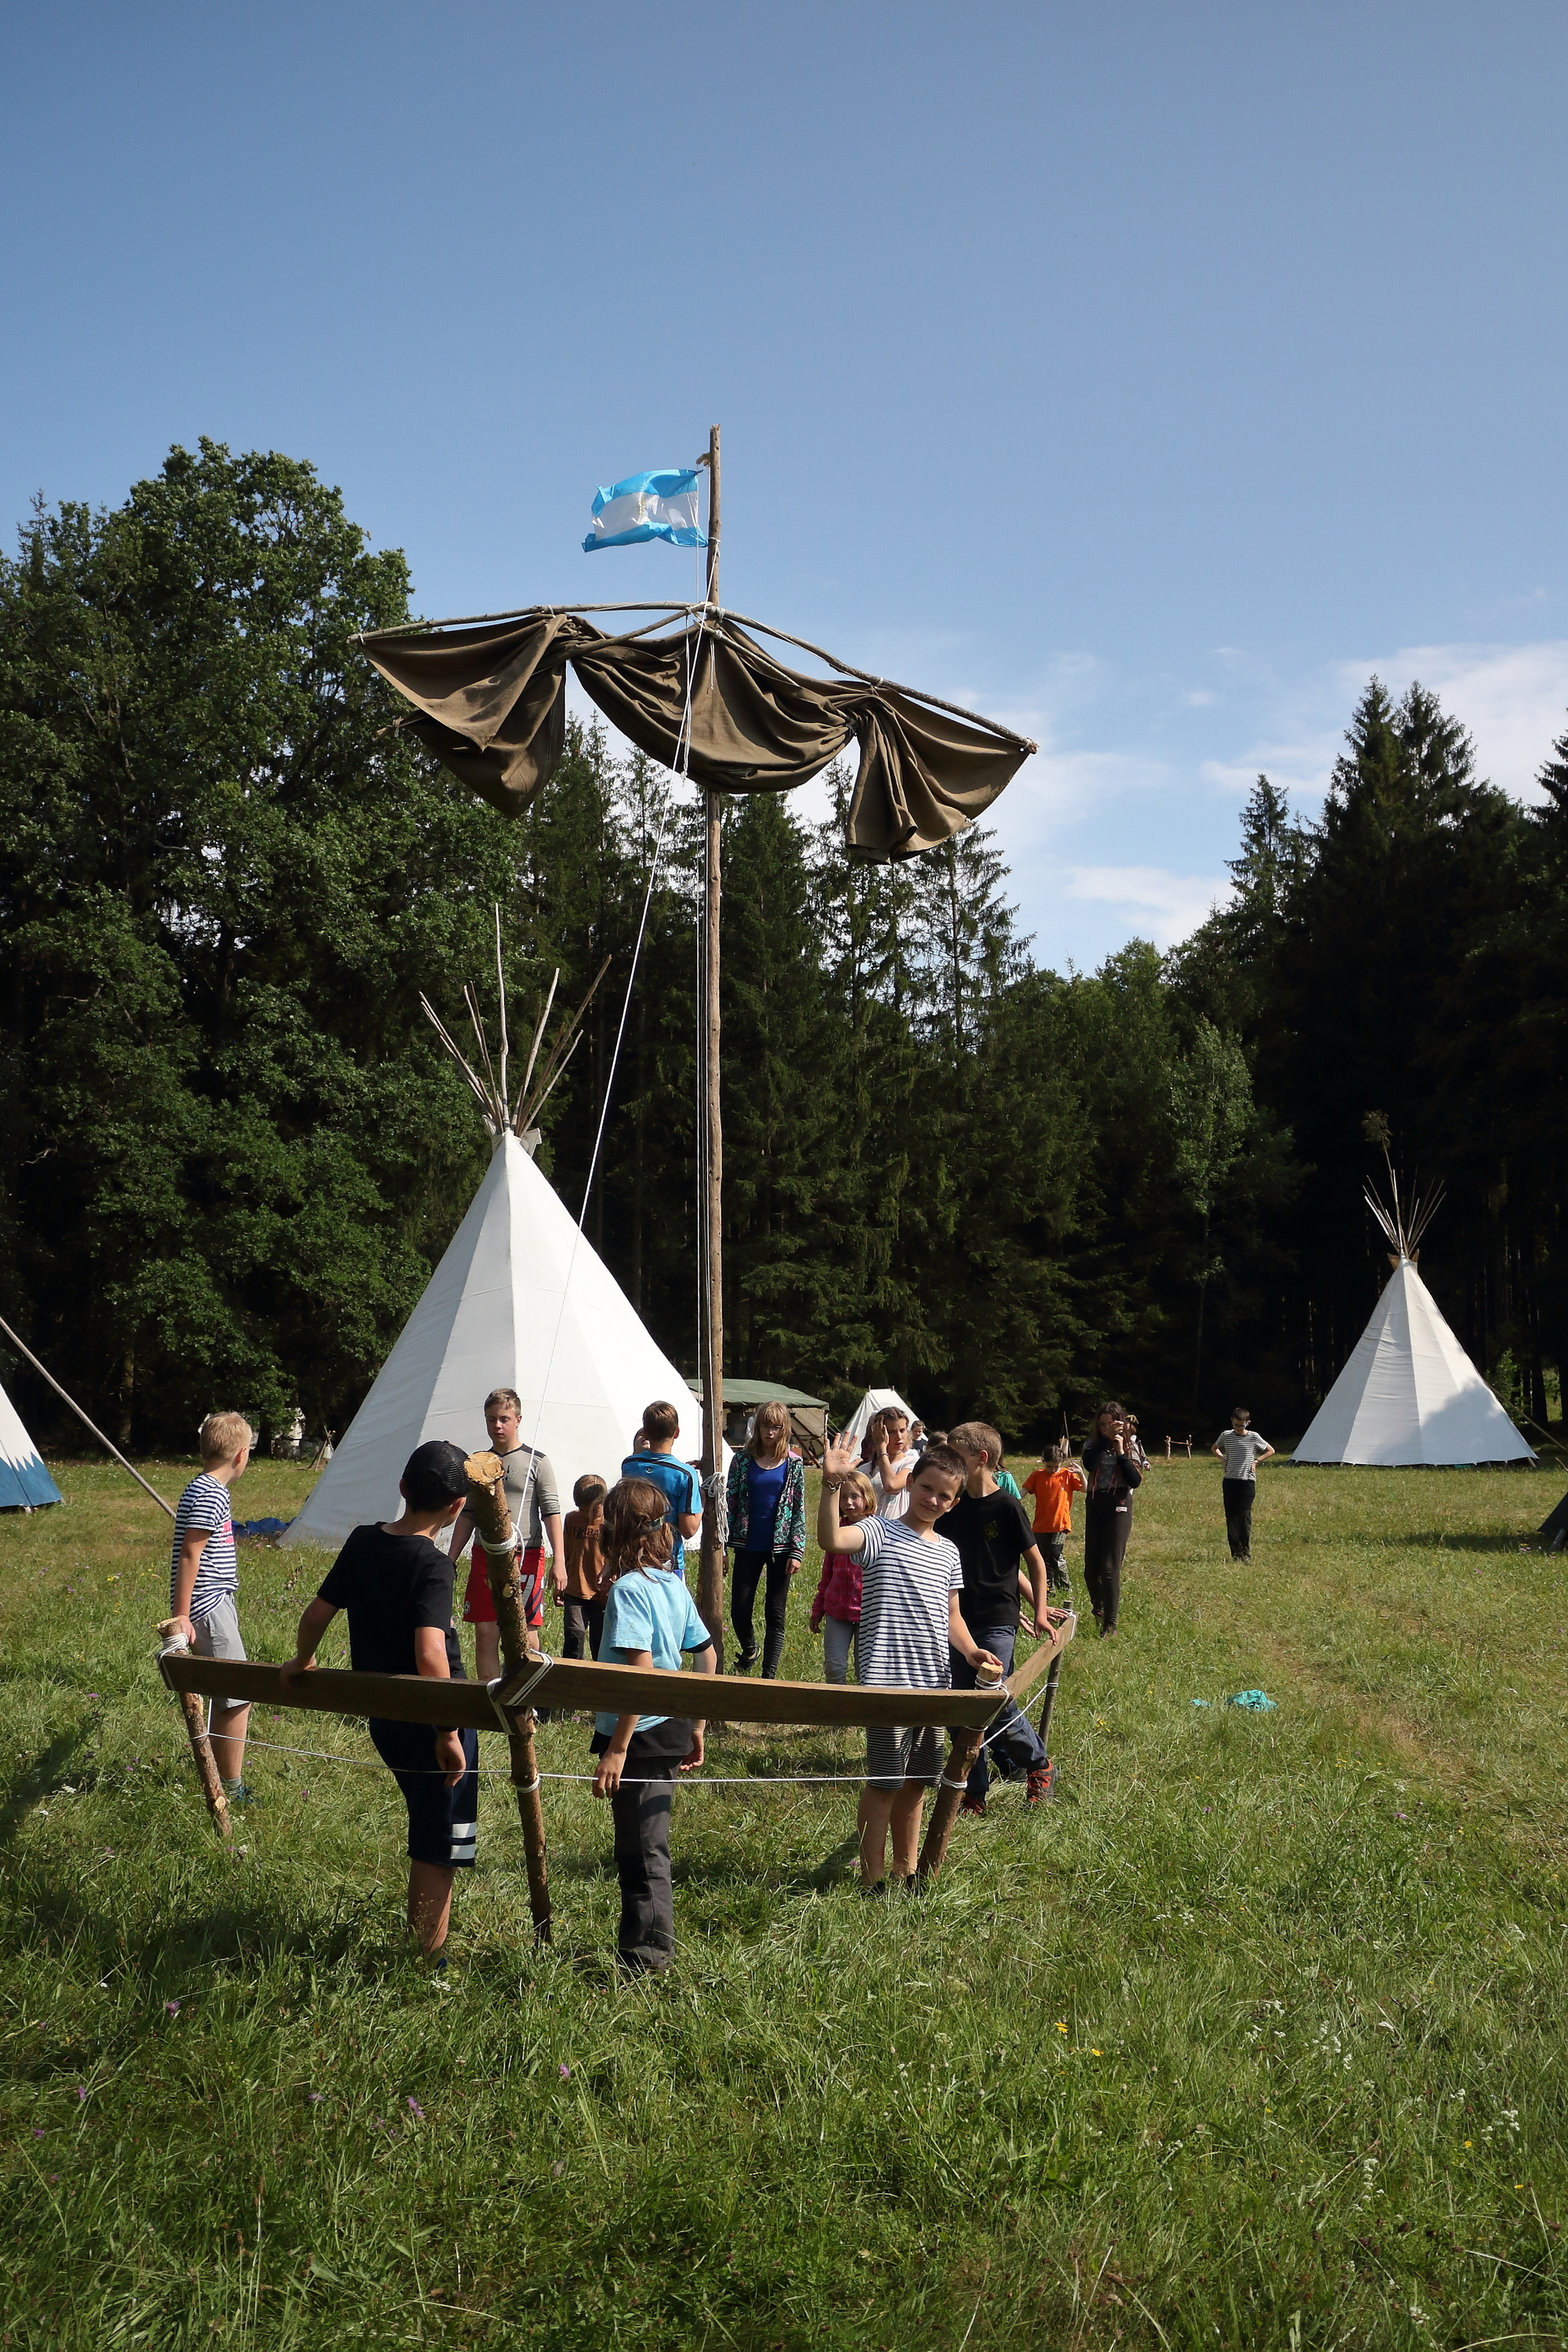
\includegraphics[width=5cm]{img/anpetu_tabor/lod.JPG}
\end{wrapfigure}
Za to, jak jsme se umístili v etapkových hrách dostáváme peníze, za které si můžeme koupit věci jako třeba plachtu nebo kotvu. Rozhodli jsme se, že si zatím nic nekoupíme.
V olympiádě bylo sedm dispcilplín. První byl hod kladivem. Mladší (Eskymáci a Kompoti) házeli myslím šestilkilovým a starší (Borúwky a Urzoni) osmikilovým. Další disciplína byla stání na jedné noze na kůlu nebo běh s uvázáním loďáku.
Taky jsme měli třeba zvonit na rolničky uvázané na stromě nebo lovit Humrovi „peníze“ z bahna.
U Vrtule jsme luštili zprávy v morseovce a pak jsme mohli i vypít ešus s vodou a běžet.

\podpis{Anežka}
% subsubsection středa_12_7_2019_olympiáda_ještě_jedna_věc (end)

\subsubsection{Noční hra} % (fold)
\label{sub:noční_hra}

začalo to tak že vedoucí hrozně moc řvali přepad vyšichni jsme vylezli ze svích tee-pee a zjistili jsme že je to noční hra museli jsme si na brat do hrníčku vodu z kíble a běžet do lesa a tam byli čtiři ohně piráti nám zapálili lodě a mi jsme je museli uhasit za ohněm byli naše věci a museli jsme je na sto procet rozeznat což nám nešlo protože jsme neměli baterku ale nakonec jsme to zvádi sice jsme byli poslední ale zvládli jsme to. :-)

\podpis{GRIZZLY}

% subsubsection noční_hra (end)

\subsubsection{Etapková hra} % (fold)
\label{ssub:etapková_hra}
	
dnes jsme se všechny skupinky sešli před ohništěm a vyděli jsme tam lidojedi žvatlali hrozně richle nějaký nesmysli: švol ky la sumture a tak dále pak jsme šli do lesa ta tam byl šaman a překlad všech divnejch slov po chvíli jsme zistili že tam všechna slova nejsou a tak jsem se zeptali šamana a ten nám to sice nějak ale moc nevisvětlil nakonec jsme si slova nějak odvodili a měli jsme to skoro správně a měli jsme to první překlad vypadal nějak takhle: mi přicházíme v míru náš kmen váš kompas ugrilují vy se budete jen dívat napijte se s námi našeho pití

\podpis{Grizzly}
% subsubsection etapková_hra (end)

\subsubsection{Honění bizonů a buvolů} % (fold)
\label{ssub:honění_bizonů_a_buvolů}

zjistili jsme že nemáme žádné zásobi tak jsme zakotvili na ostrově kde jsme si byli jstí že tam jídlo bude ale nebylo ukázali nám papír na kterém měli plán a ten plán znamenal že nemají jídlo tak jsme museli chytat Bizoni a bůvoli a měli bysmé jich mít stejně a měli jsme mít dvojice ve tkerých jsme honili udi a bylo to tak že se ho musí dotknout oba ale jakmile se ho jeden dotkne tak bůvol – nebo byzon začne počíta a utíka a když ho druhý člen tímu nechytí musí se jít oživit a když ho chytne bůvol – nebo byzon jim vydá papírek mi jsme skončili jako třetí protože jsme měli výde bizonů

\podpis{Grizzly}
\begin{center}
	\includegraphics[width=12cm]{img/anpetu_tabor/hra.jpg}
\end{center}

% subsubsection honění_bizonů_a_buvolů (end)

\subsubsection{Cestování lodí} % (fold)
\label{ssub:cestování_lodí}

šli jsme do lesa a tam jsme vyděli několik lodí/udů udové měli šátky a běhali k jinému stromu na kterém byl papír třeba srí lanka a uďa který jel na srí lanku tak potřeboval peníze na suroviny a další věci a mi jsme mu mohli půjčit peníze a když na lanku doje se šátkem tak nám dal dvojnásobek nebo 3x nebo někdy 4x a ostatní co přispívali na lodě mohli někomu uďovi vzít šátek a jakmile uďa stratí šátek tak loď skrachuje a všechny peníze co jsme na loď vsadili propadli měli jsme každý 200 Kč a většina skončila cca u 1000 Kč

\podpis{Grizzly}
% subsubsection cestování_lodí (end)

\subsubsection{Bar} % (fold)
\label{ssub:bar}
setkali jsme se s Hanjetu u jídelny která byla zakrytá dekama a unit byli různý uďové/námořníci který se s námi o něco vsadili a když jsme vyhráli tak nám dali peníze a kdy jsme prohráli tak nám vzali peníze a za peníze jse si mohli koupit různý moc dobrý věci čokoládu, sušenky a další různý šladkosti nebo jsme si mohli vydělat peníze jinou cestou někdo někoho pocozí na dvojkoláku, namasíruje a tak dále

\podpis{Grizzly}
% subsubsection bar (end)

\subsubsection{Manévry} % (fold)
\label{ssub:manévry}

Nej dřív jsme šly k rybníku a tam se vibourala loď a potom sm šli do ostrovce a tam k rybníku kde byl papírek a od tam tud sme šli k dalšímu papírku, až jsme došli do nějaké vesnice, kde na nás čekali Vrtule a Humr. S nima jsme přespali mezi rybníkama Vosovice a Žabák. Ráno jsme vyrazili k rybníku Zhoř, kde jsme u stavidla našli papírek v morseovce.

Dál jsme šli do Nevězic přes nějakou vesnici, kde jsme měli počítat dřevěná zvířata. V Nevězicích jsme se naobědvali a pokračovali jsme k rozcestníku Luh. Od tamtuď jsme šli k rozcestníku Lipice, který byl asi 8 km od Luhu. Cestou jsme šli přes nějakou vesnici, kde nám jedna paní doplnila vodu a navíc nám dala i bonbóny. Potom jsme šli k mostu přes řeku, kde byli uďové a oznámení, že se zítra na hradě Zvíkov sejdou piráti, a že pokud chceme pomoct, že se máme ráno mezi 9:00 a 10:00. Tak jsme zamířili k lesu pobíž hradu, kde jsme se potkali se skupinkou Plejtváci a Borci. Ráno jsme šli na hrad, kde jsme potkali piráta Strniště jehož deník byly ty papírky, co jsme nacházeli.

Ten nám řekl místo, kde byla schovaná mapa (část) k pokladu Žaka Hnědovouse. Pak jsme se vraceli do tábora a byli jsme první!

\podpis{Anežka}
\begin{center}
	\includegraphics[width=8cm]{img/anpetu_tabor/pirati.JPG}
\end{center}

% subsubsection manévry (end)

\subsubsection{Etapková hra} % (fold)
\label{ssub:etapková_hra1}

Sice jsme získali mapu, jenže na ní není zakreslené místo, kde se nachází poklad.

Takže jsme měli na louce najít naše piráty a získat od nich tři indície, které pak spojily všechny skupinky dohromady a vyšly z toho „souřadnice“ pokladu.

\podpis{Anežka}


Nakonec jsme zjistili, že je to mapa NEPROBÁDANÝCH ÚZEMÍ.

\begin{center}
	\includegraphics[width=10cm]{img/anpetu_tabor/svojsik.jpg}
\end{center}

% subsubsection etapková_hra (end)

\subsubsection{Etapková hra} % (fold)
\label{ssub:etapková_hra2}

kapitínce kukumbrii se stratil papoušek a dalších spousu věci tak jsme šli na viznačené místo kde ty věci jsou a mi jsme si museli nakreslit mapu abychom věděli kde ti věci jsou a mohli tam doplout našli jsme tam například, tužku, sprej, vlajku nebo něco takového. Když jsme měli všechno zapsáno (nelbo ono jsme na to měli určitý čas ta-takže jsme měli co jsme měli ale byl to dostateční čas) tak jsme pak šli do tábora

\podpis{GRIZZLY}
% subsubsection etapková_hra (end)

\subsubsection{Vařící etapka} % (fold)
\label{ssub:vařící_etapka}

Uďové nám oznámili, že máme uvařit pro Kukumbrii oběd, protože bude mít teď někdy narozeniny. Rozhodli jsme se, že budeme vařit v Borúwčím týpku, kam jsme si začali nosit suroviny na hodněchodový oběd pro Kukumbrii. Nakonec jsme měli: 1 rajče, skoro celou okurku, pytlík mouky, 7 brambor, 1 krajíc chleba, 5 vajíček, olej, sůl, koření, a hlavně rybu. Byla to ryba která měla hodně kostí, takže jsme měli takové maké kousíčky, které jsme smíchali s vajíčkem a moukou. Taky jsme se pokoušeli osmažit hranolky, ake nakonec jsme je rozmačkali na kaši, chutnaly tak líp. Taky jsme udělali jako přílohu chleba ve vajíčku. Kukumbrie řekla, že je to dobré.

\podpis{Anežka}
\begin{center}
	\includegraphics[width=8cm]{img/anpetu_tabor/vorvo.JPG}
\end{center}

% subsubsection vařící_etapka (end)
\subsubsection{Bar} % (fold)
\label{ssub:bar1}

kapitánka Kukumbrie měla narozeniny a tak musela být oslava dali jsme ji dárky: píšťalku, míček, tučňáka, čokoládu a bonbóny. pak byl bar jako takový: překecávaná, sirky, kolíčky a hlavně sladkosti a slavnosti.:-) Pak jsme šli ven protože jsme slišeli romantickou hudbu a tam byla kukuočko s Eulálií na lodi a bylo to jako v titaniku

\podpis{GRIZZLY}

% subsubsection bar (end)

\subsubsection{Vyvražďování} % (fold)
\label{ssub:vyvražďování}

kapitánka kukumbrie drsné oko měla mít narozeniny a protože je to skvělá kapitánka tak jsme prostě museli mít dárek a přáníčko tak jsme dostali seznam věcí co máme sehnat a vyrazili jsme abychom to stihli šli jsme do vesnice a tam jsme museli sehnat: nejoriginálnějsí vec k narozeninám, přáníčko a dort nebo jinou pochutinu (pak taky jsme měli sechnat ten dárek tak že si budeme vyměňovat mušličku) a do tábora jsme měli dojít nejpozději v 19:00 vše jsme stihli a dostali jsme spóóóusti věcí a dobrot:-)

\podpis{Grizzly}

\begin{center}
	\includegraphics[width=12cm]{img/anpetu_tabor/taborak.JPG}
\end{center}

% subsubsection vyvražďování (end)
\subsubsection{Pokladovka} % (fold)
\label{ssub:pokladovka}

přepadli nás piráti a zabili kukumbrrii pak nás hned vyslali pomstít kukumbrii a najít poklad poslali nás do ostrovce na poštu kde vjsme měli najít čtiři obáli se jmény etapek v obálkách bylo napsáno v šivře ke je poklad (v šifrě) tak jsme tak došli a tam byla další správa o tom že si z nás vystřelili přesněji napsáno ha, ha napálili jste se hlupáci jen jsme získali čas na zakopání pokladu vraťe se do tábora Jonatán nám naštěstí řekl kde je poklas a museli jsme procházet tábořiště domorodců a pak jsme přešli rybník k ostrůvku kde byli piráti kteří po nás začali střílet naštěstí jsme mohli používat jejich papírové koule které používali jako střelbu a pomalu slábli a slábli až umřeli pak jsme našli místo kde by mohl být poklad a vykopali jsme ho tam bylo egzotické ovoce tak jsme ho vzali do tábora kde byla supr hostina: řízky, okurky, papryky, rajčátka a tak dále a protože jsme přijeli hodně pozdě tak jsme zalezli do sPacáčků a spali Grizzly a Karkulka


% subsubsection pokladovka (end)
% chapter lodní_deník_etapkové_skupiny_černí_rytíři_anpetu_ (end)

\begin{center}
	\includegraphics[width=\textwidth]{img/anpetu_tabor/spolecna.JPG}
\end{center}
\clearpage